\section{Integration und Programmierung der Steuerungstechnik \textcolor{gray}{ (Vincent Sonvilla)}}


\subsection{Aufgabenstellung}

\subsection{Tia-Portal Grundlagen}

Tia Portal (Totally Integrated Automation Portal) ist die zentrale Software von Siemens zur Programmierung, Konfiguration und Diagnose von Automatisierungssystemen. Es ermöglicht die Steuerung von SPS (Speicherprogrammierbare Steuerungen), HMI (Bedienpanels) und Antrieben in einer einzigen Umgebung.

    \subsubsection{Programm erstellen}

    \subsubsection{Programmbausteine}
    
    In TIA Portal werden Programmbausteine genutzt, um Steuerungsprogramme modular und strukturiert zu gestalten. Dadurch werden Programme übersichtlicher, wiederverwendbar und effizienter. Es gibt unterschiedliche Arten von Programmierbausteinen:

    \begin{itemize}
        \item[1.] OB(Organisationsbausteine)
            Organisationsbausteine werden verwendet um das Anwenderprogramm hierarchisch zu strukturieren. Auch für OBs stehen,wie in Abb. \ref{Organisationsbausteine} gezeigt, unterchiedliche Bausteine zur Verfügung:
            \begin{figure}[h]
                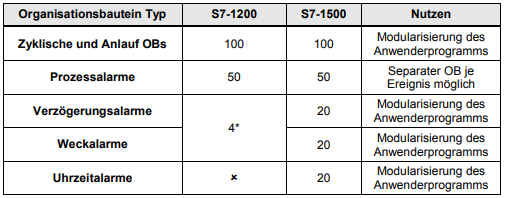
\includegraphics[width=\textwidth]{Sonne/Tia-Portal_Organisationsbausteine.png}
                \caption{Organisationsbausteine}
                \label{Organisationsbausteine}
            \end{figure}
    \end{itemize}

    \subsubsection{Technologieobjekte}

    \subsubsection{Programmiersprachen}

    \subsubsection{Librarys}
    \label{Libraryeinbindung}

\subsection{Motorenansteuerung}

\subsection{SPS-Server Kommunikation}

    \subsubsection{Zur Auswahl stehende Kommunikationsprotokolle} 
    \label{Kommunikationsprotokolle}

    Kommunikationsprotokolle ermöglichen den Datenaustausch zwischen unterschiedlichen Systemen, indem sie Standards und Regeln für die Kommunikation definieren. In diesem Projekt wurden zwei Protokolle getestet und miteinander verglichen: OPC-UA sowie das HTTP-Protokoll.


         \paragraph{Allgemeines}

        \begin{itemize}
            \item \textbf{HTTP (Hypertext Transfer Protocol):}  \mbox{} \\
            HTTP ist eines der bekanntesten Protokolle, welches für die Datenübertragung zwischen Clients und Servern verwendet wird. Es basiert auf einem Anforderungs-Antwort-Prinzip, bei dem ein Client (Bsp.: Webbrowser) Anfragen an einen Server sendet, welcher anschließend die entsprechenden Daten zurückschickt. Die Anfrage wird als HTTP Request und die Antwort als HTTP Response bezeichnet.\cite{HTTP-Allgemein}
            
            \item \textbf{OPC-UA (Open Platform Communications - Unified Architecture):} \mbox{} \\
            OPC-UA (Open Platform Communications Unified Architecture) ist ein plattformunabhängiges Kommunikationsprotokoll, das speziell für industrielle Anwendungen entwickelt wurde. Es ermöglicht eine herstellerunabhängige Kommunikation zwischen verschiedenen Geräten bzw. Systemen. \cite{OPC-UA}
        \end{itemize}

        \paragraph{Funktionsweise}

            \begin{itemize}
                \item \textbf{{HTTP (Hypertext Transfer Protocol):}} \mbox{} \\
                
            
                \item \textbf{{OPC-UA (Open Platform Communications - Unified Architecture):}} \mbox{} \\
                
            \end{itemize}
        
            

    
    \subsubsection{Verbindungsherstellung}
    Aus den in Punkt \ref{Kommunikationsprotokolle} genannten Gründen wurde das HTTP Protokoll ausgewählt. Um in TIA-Portal die Verbindung via HTTP aufzubauen, benötigt man bestimmte Libraries die von Siemens zu Verfügung gestellt werden. Diese müssen dann wie im Punkt \ref{Libraryeinbindung} gezeigt eingebunden werden, um die Funktionsbausteine der Library nutzen zu können. 

        \paragraph{Funktionsbausteine} \mbox{} \\
        In der Library stehen dann folgende Bausteine zur Verfügung:

        \begin{itemize}
            \item GET
            \item POST-PUT \\
            Mit dem POST-PUT Befehl werden Daten zum Server geschickt aber auch Daten erhalten. 
        \end{itemize}


    \subsubsection{Datenfilterung}
    Die vom Server geschickten Daten werden in einem Befehl geschickt. Aus diesem Befehl muss herausgelesen werden um welche Aufgabe es sich handelt, und die Daten die erforderlich sind um diesen Befehl auszuführen.

        \paragraph{Datenformatierung}\mbox{}\\
        Die Daten werden in einem String geschickt, welcher in zwei Teile aufgeteilt wird. Der zweite Teil ist jedoch abhängig vom ersten. \\
        
        \begin{itemize}
            \item 1.Teil: \\
            IDXXXXAXX \\
            Aus diesem Teil werden die ID-Nummer sowie der Auftrag herausgefiltert. Die ID-Nummer ist eine 4 stellige Nummer welche nach ID steht. Der Auftrag welcher ausgeführt werden muss steht in den zwei Stellen nach A.\\
            Diese werden nach folgender Codierung ausgelesen:
                \subitem 00: Kommissionierstation
                \subitem 01: Förderband
                \subitem 10: Lager 1 (Aus-/Einlagerung)
                \subitem 11: Lager 1 (Querförderer)
            \item 2.Teil: \\
            Der zweite Teil steht in Abhängigkeit zu ersten. Je nachdem welche Zahl nach A steht,also der Code welche Area angesprochen wird, ist der zweite Teil anders aufgebaut.
                \begin{itemize}
                \item 00: 
                \item 01:
                \item{10: X-Position, Y-Position, Z-Position,Ein/-Auslagerung \\
                Wobei nach jedem Symbol eine 4 stellige Zahl steht.Also X0000Y0000Z0000R0 bedeutet, dass die 
                X-Position 0, Y-Position 0, Z-Position 0 und es sich um eine Auslagerung handelt.}
                \item 11:
                
                \end{itemize}
            
        \end{itemize}

\subsection{Herausforderungen}
